% Introduction

% Main chapter title
\chapter{Modification in Min Sum Algorithm using partitioning}

% Change X to a consecutive number; for referencing this chapter elsewhere, use \ref{ChapterX}
\label{Chapter7} 

% This is for the header on each page
\lhead{Chapter 6. \emph{Proposed modification in Min Sum Algorithm using partitioning}}  

The idea is to modify the min sum algorithm such that we can deploy it in a partitioned matrix iteratively to decode a code block.
To state the modification we first explain min sum algorithm by a example and then we show the modification in it:

\section{Example explaining min sum decode }
The parity check matrix chosen to decode the code block is as following.
\[
\left[ \begin{array} {c|cccccccc} 
  &    c1 &   c2 &   c3 &  c4  &  c5  &  c6  &  c7  &  c8 \\ \hline
r1 &    1  &   1  &   1  &   0  &   0  &   0  &   0  &   0 \\
r2 &    0  &   0  &   0  &   1  &   1  &   1  &   0  &   0 \\ 
r3 &    1  &   0  &   0  &   1  &   0  &   0  &   1  &   0 \\
r4 &    0  &   1  &   0  &   0  &   1  &   0  &   0  &   1 \end{array} \right] 
\]			
The Tanner graph corresponding to above parity check  matrix is depicted in figure \ref{Tanner Graph}.
\\
\begin{figure}[h!]
\centering
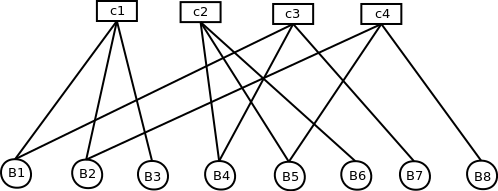
\includegraphics[height=5cm,width=12cm]{minSum1}
\caption[Tanner Graph]{Tanner Graph}
\label{Tanner Graph}
\end{figure}

The code block received at the receiver is represented by C. The SNR at the input of receiver is represented as $\dfrac{E_{b}}{No}$. The code is represented as R.
\\
\textbf{Step 1:} We calculate the a priori probabilities at the receiver end. A priori probability of a particular code bit is the log likelyhood ratio of the code bit.
\[  aPriori[I] = -4 * C[I] * R * \dfrac{Eb}{No} \]
Assuming we get the a priori probability = \{ -3.2 , 2.8 , -3.6 , 2.8 , 2 , -6 , - 9.6 , -4.8 \}
\begin{figure}[h!]
\centering
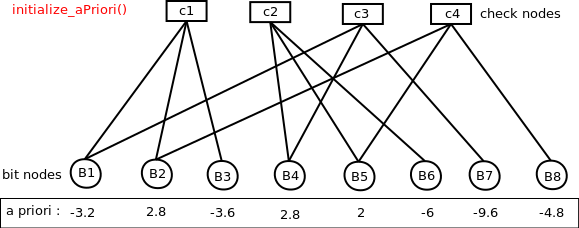
\includegraphics[height=6cm,width=12cm]{minSum2}
\caption[Initialization of a priori probabilities ]{Initializing a priori probabilities}
\label{minSum2}
\end{figure}
\\
\textbf{Step 2:}
We calculate messages transferred from bit nodes to check nodes through the edges of Tanner graph as depicted in figure \ref{minSum3}
 \[ message[I][J] = aPriori[I] \]
\begin{figure}[h!]
\centering
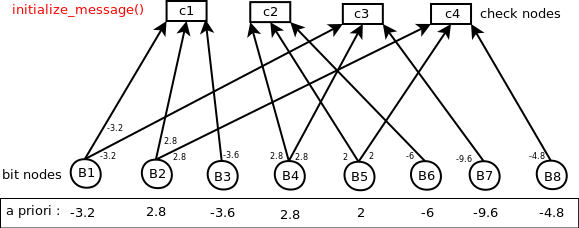
\includegraphics[height=6cm,width=12cm]{minSum3}
\caption[Initialization of messages]{Initializing messages}
\label{minSum3}
\end{figure}

\textbf{Step 3:}
We calculate extrinsic information at the check nodes and transfer the information back to the bit nodes through edges as depicted in figure \ref{minSum4}
 \[ |E_{(j,i)}| =  Min_{i'\in B_j \ i'\neq i }|M_{j,i'}|   \] 
 \[ sign({E_{(j,i)}}) =  \prod_{i'\in B_j \ i'\neq i }sign(M_{j,i'})   \]
\begin{figure}[h!]
\centering
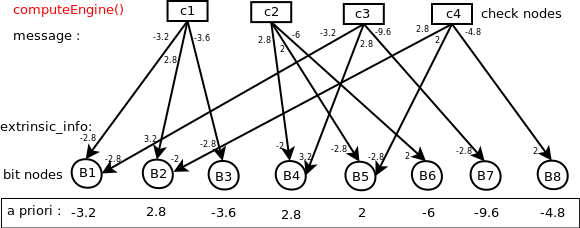
\includegraphics[height=6cm,width=12cm]{minSum4}
\caption[Computation of extrinsic information]{Computing extrinsic information}
\label{minSum4}
\end{figure}

\textbf{Step 4:}
After computation of extrinsic informations we calculate a posteriori probabilities at each bit nodes as depicted in figure \ref{minSum5}
\begin{figure}[h!]
\centering
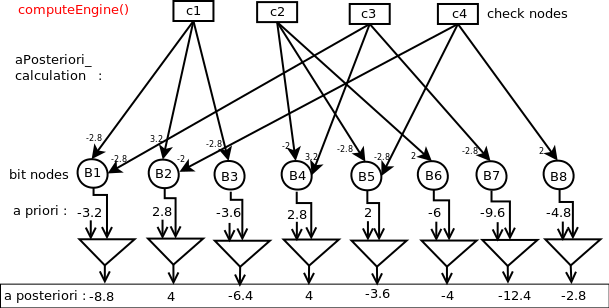
\includegraphics[height=8cm,width=12cm]{minSum5}
\caption[Calculation of a posteriori probabilities]{Calculating a posteriori probabilities}
\label{minSum5}
\end{figure}

\textbf{Step 5:}
A posteriori probabilities are the estimate of the code bits. Thus we take hard decision on the a posteriori probabilities. And this new estimate of code block is compared to the present code block. If both are same  then decoding stops. 

\textbf{Step 6:}
Else, we modify the code bits and messages and start the next iteration to decode the code block. The messages are updated as shown is figure \ref{minSum7}
\begin{figure}[h!]
\centering
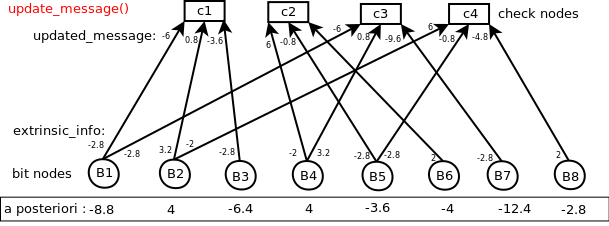
\includegraphics[height=6cm,width=12cm]{minSum7}
\caption[Updating the messages]{Updating the messages}
\label{minSum7}
\end{figure}

\section{ Example explaining modifications on min sum decode algorithm for a partitioned matrix }

As we have partitioned the matrix the parity check matrix looks as follows.
\[
H = \left[ \begin{array}{c|c}  
H11  & H12     \\ \hline
H21  & H22     \end{array} \right] 
\] 
\[
\left[ \begin{array} {c|cccccccc} 
  &    c1 &   c2 &   c3 &  c4  &  c5  &  c6  &  c7  &  c8 \\ \hline
r1 &    1  &   1  &   1  &   0  &   0  &   0  &   0  &   0 \\
r2 &    0  &   0  &   0  &   1  &   1  &   1  &   0  &   0 \\ 
r3 &    1  &   0  &   0  &   1  &   0  &   0  &   1  &   0 \\
r4 &    0  &   1  &   0  &   0  &   1  &   0  &   0  &   1 \end{array} \right] 
     \Rightarrow
\left[ \begin{array} {c|cccc|cccc} 
  &    c4 &   c6 &   c7 &  c1  &  c2  &  c3  &  c8  &  c5 \\ \hline  
r2 &     1  &   1  &   0  &   0  &   0  &   0  &   0  &   1 \\
r3 &     1  &   0  &   1  &   1  &   0  &   0  &   0  &   0 \\ \hline
r1 &     0  &   0  &   0  &   1  &   1  &   1  &   0  &   0 \\
r4 &     0  &   0  &   0  &   0  &   1  &   0  &   1  &   1 \end{array} \right] 
\]

\textbf{Step 1:} 
Assuming we get the a priori probabilities = \{ 5.59 , -11.99 , -19.19 , -6.39 , 5.59 , -7.1 , - 9.59 , 3.99 \}. The a priori initialization is shown in figure \ref{minSumModified1}
\begin{figure}[h!]
\centering
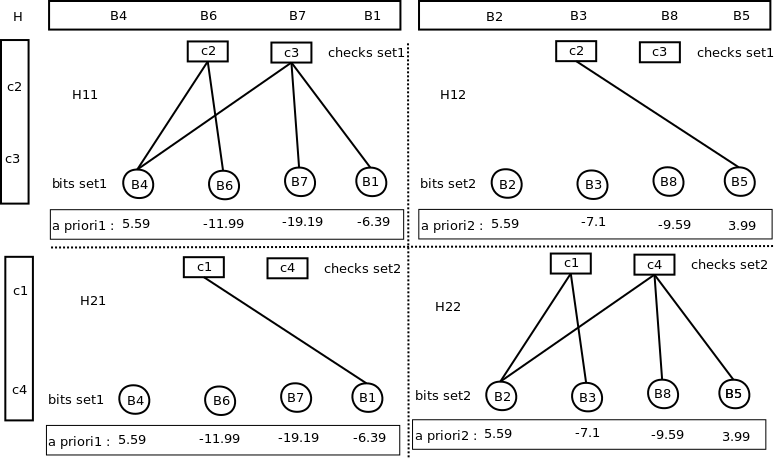
\includegraphics[height=8cm,width=12cm]{minSumModified1}
\caption[Initialization of a priori probabilities on  partitioned Tanner graphs]{Initializing a priori probabilities on partitioned Tanner graphs}
\label{minSumModified1}
\end{figure}
\\
\textbf{Step 2:}
The message initialization is done similarly and is  depicted in figure \ref{minSumModified2}
\begin{figure}[h!]
\centering
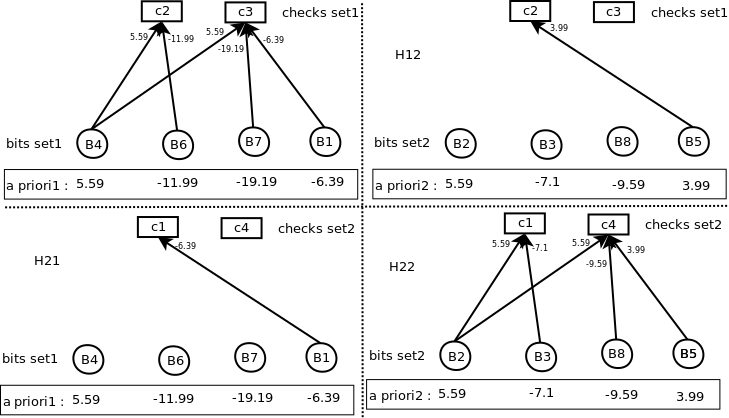
\includegraphics[height=8cm,width=12cm]{minSumModified2}
\caption[Initialization of messages on  partitioned Tanner graphs]{Initializing messages on  partitioned Tanner graphs}
\label{minSumModified2}
\end{figure}
\\
\textbf{Step 3:}
The computation of extrinsic information is broken into two parts. First we calculate partial extrinsic information at each matrix separately. At the same time we compute the transverse information required to calculate complete information from one check matrix to other check matrix, as depicted in figure  \ref{minSumModified3}

\begin{figure}[h!]
\centering
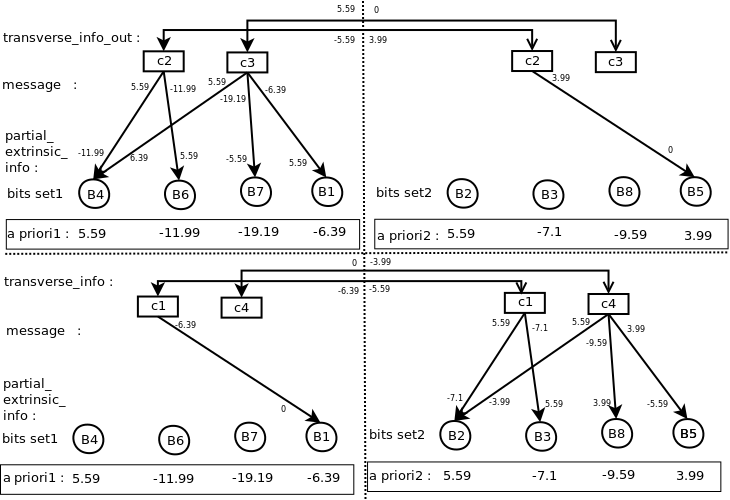
\includegraphics[height=8cm,width=12cm]{minSumModified3}
\caption[Computation of partial extrinsic information \& Transverse information ]{Computing partial extrinsic information \& Transverse information}
\label{minSumModified3}
\end{figure}

\textbf{Step 4:}
Then extrinsic information computation is completed by the transverse information as depicted in figure \ref{minSumModified4}
\begin{figure}[h!]
\centering
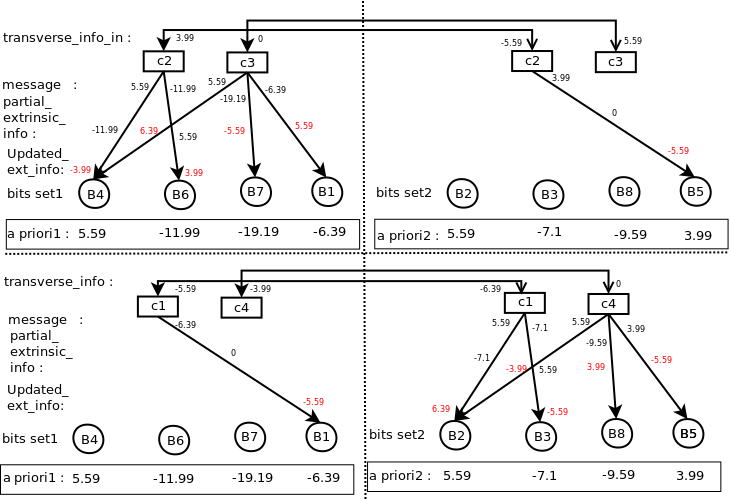
\includegraphics[height=8cm,width=12cm]{minSumModified4}
\caption[Computation of extrinsic information using Transverse information]{Computing extrinsic information using Transverse information}
\label{minSumModified4}
\end{figure}

\textbf{Step 5:}
A posteriori probabilities are  calculated similarly and the following steps of the algorithms remain the same. 

\section{ Modified Min Sum Algorithm }

By partitioning the matrix we can start computation in each matrix in parallel. This gives the hopes to parallelize the system and reduce the overall computation time. But the problem is that the computation on the partitioned matrix is not totally independent of the other matrices. Thus, the goal is to reduce the overall dependency of the computation in one partition of the matrix with the other partition of the matrix. The results after partitioning are shown in chapter 6 .The results are promising to get the desired behaviour. \\

The modification is essentially breaking the computation of extrinsic informations into multiple parts. The example explained that for a two way partition we have to break the computation in two stages. Similarly for a n-way partition we can break the computation in n stages. The trade off lies between number of stages and the number of computation engines. \\

For a two way partitioned matrix, the extrinsic information calculation is broken into two stages as following.
\\
\textbf{Stage 1:}
Partial extrinsic informations are calculated as for every matrix as following :
\begin{align}
|Ep_{(j,i)}| =  Min_{i'\in B_j \ i'\neq i }|M_{j,i'}|                                                                 
\end{align} 

\begin{align}
 sign({Ep_{(j,i)}}) =  \prod_{i'\in B_j \ i'\neq i }sign(M_{j,i'})  
\end{align} 
And the transverse corrections are calculated as following :

Transverse corrections is the information transferred between computation engines that shares common check nodes. Thus, these are computed for each check node. 
\begin{align} |T_{(j)}| =  Min_{i'\in B_j }|M_{(j,i')}|  
\end{align}  
\begin{align} sign({T_{(j)}}) =  \prod_{i'\in B_j}sign(M_{(j,i')})  
\end{align} 
 
\textbf{Stage 2:}
By using transverse information we calculate the net extrinsic information. 
\begin{align} |E_{(j,i)}| =  Min {|Ep_{(j,i')}| ,|T_{(j)}| }  
\end{align} 
\begin{align} sign({E_{(j,i)}}) =  \prod{sign(Ep_{(j,i')},sign(T_{(j)})  }
\end{align} 

Just keep in mind extrinsic information of a particular check node in a particular matrix depends upon partial extrinsic information of the same check node calculated in stage 1 by the same matrix, but transverse information of the matrix that shares the common check node. \\
As explained in the above example transverse information is transferred from $H_{(1,1)}$ to $H_{(1,2)}$ and vice versa. Similarly from  $H_{(2,1)}$ to $H_{(2,2)}$ and vice versa to compute the overall extrinsic information. \\

Thus if we generalise the concept for n-way partitioned matrix we just need to calculate the partial extrinsic information in stage 1. And then in subsequent stages we have to take in account the transverse information computed by same check node in all other n-1 partitioned matrices, that shares common check node. Thus we need a total number of n stages for a n-way partitioned matrix.

